\documentclass{article}

\usepackage[scientific-notation=true, binary-units=true]{siunitx}
\sisetup{per-mode=fraction}%
\sisetup{scientific-notation=false}%
\usepackage{amsmath}
\usepackage{forest}

\usepackage{tikz}
\usetikzlibrary{shapes,arrows}
\usetikzlibrary{positioning}

\tikzstyle{block} = [rectangle, draw, fill=white!20, 
     text centered, rounded corners, minimum height=3em]
\tikzstyle{blob} = [circle, draw, fill=white!20, 
    text width=2em, text centered, rounded corners, minimum height=2em]
\tikzstyle{cloud} = [draw, ellipse,fill=white!20, node distance=3cm,
    minimum height=2em]
\tikzstyle{arrow} = [thick,->,>=stealth]

\title{SYSC 4502 Assignment 4}
\date{April 7th, 2017}
\author{Jessica Morris \(100882290\)}

\begin{document}

\maketitle

\begin{enumerate}

\item
\begin{enumerate}

\item The output will be 00000101 repeated eight times.

\item The output will be 00000101 repeated seven times, ended with 10000101.

\item For (a), the output will be 10100000 repeated eight times. For (b), the output will be 10000101 followed by 
10100000 repeated seven times.

\end{enumerate}

\item
\begin{enumerate}

\item $ n = p \times q = 5 \times 11 = 55 $, $ z = (p-1)(q-1) = 4 \times 10 = 40 $

\item $ e = 3 $ is acceptable because it is less than $n$, and has no common factors with $z$.

\item $$ de = 1(\text{mod } z) $$
$$ 3d = 1(\text{mod } 40) $$
$$ d = \frac{1(\text{mod } 40)}{3} $$
The nearest integer that gives $ x = 1(\text{mod } 40) $ and is divisible by 3 is 81. Therefore:
$$ d = \frac{81}{3} $$
$$ d = 27 $$

\item For $ m = 8 $, the ciphertext $c$ is:
$$ c = m^e \text{mod } n $$
$$ c = 8^3 \text{mod } 55 $$
$$ c = 512 \text{mod } 55 $$
$$ c = 17 $$

\end{enumerate}

\item Bob's steps to decode the package from Alice:

\hspace*{-2cm}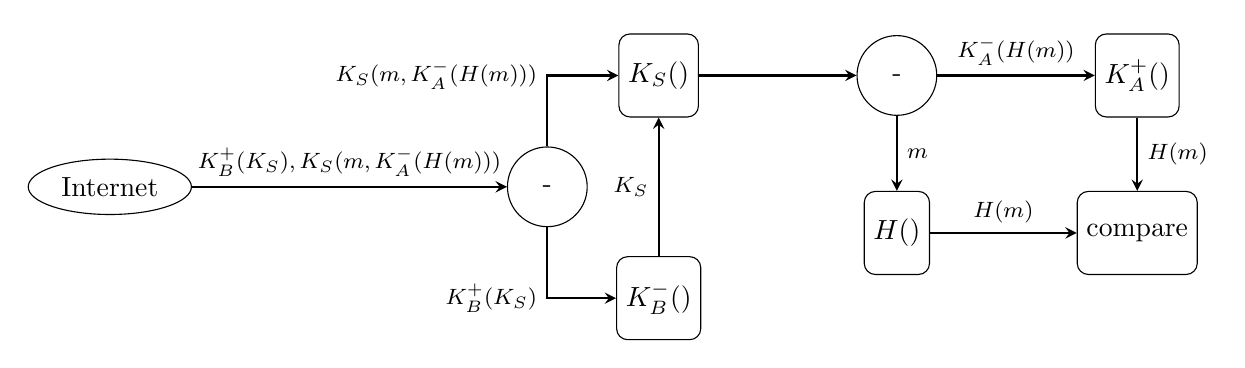
\begin{tikzpicture}[node distance = 2cm, auto]
    % Place nodes
    \node [cloud] (internet) {Internet};
    \node [blob, right=4cm of internet] (sub1) {-};
    \node [block, above right of=sub1] (ks) {$K_S()$};
    \node [block, below right of=sub1] (kb) {$K_B^-()$};
    \node [blob, right=2cm of ks] (sub2) {-};
    \node [block, below of=sub2] (h) {$H()$};
    \node [block, right=2cm of sub2] (ka) {$K_A^+()$};
    \node [block, below of=ka] (compare) {compare};
    
    % Draw edges
    \draw [arrow] (internet) -- node {\footnotesize $K_B^+(K_S),K_S(m,K_A^-(H(m)))$} (sub1);
    \draw [arrow] (sub1) |- node[anchor=east] {\footnotesize $K_S(m,K_A^-(H(m)))$} (ks);
    \draw [arrow] (sub1) |- node[anchor=east] {\footnotesize $K_B^+(K_S)$} (kb);
    \draw [arrow] (kb) -- node {\footnotesize $K_S$} (ks);
    \draw [arrow] (ks) -- (sub2);
    \draw [arrow] (sub2) -- node {\footnotesize $m$} (h);
    \draw [arrow] (sub2) -- node {\footnotesize $K_A^-(H(m))$} (ka);
    \draw [arrow] (h) -- node {\footnotesize $H(m)$} (compare);
    \draw [arrow] (ka) -- node {\footnotesize $H(m)$} (compare);
\end{tikzpicture}

\item
\begin{enumerate}

\item The three fields are (ICV = 1010 pre-encryption):

\begin{tabular}{|c|c|}
    \hline
    IV & 11 \\ \hline
    message &  \\ \hline
    ICV & 1010 \\ \hline
\end{tabular}

\item b

\item c

\item d

\end{enumerate}

\item Grid-of-Tries: 

\begin{forest}
for tree={circle,draw, l sep=20pt, s sep=20pt}
[ 
    [ ,edge label={node[midway,left] {0}}   
      [ ,edge label={node[midway,left] {0}}
        [ ,edge=dashed]
      ]
      [ ,edge=dashed]
    ]
    [ ,edge=dashed]
    [ ,edge label={node[midway,right] {1}} 
     [ ,edge label={node[midway,left] {0}}
       [ ,edge label={node[midway,left] {0}}
         [ ,edge label={node[midway,right] {1}}
           [ ,edge=dashed]
         ]
       ]
       [ ,edge=dashed]
       [ ,edge label={node[midway,right] {1}}
         [ ,edge=dashed]
       ]
     ]
     [ ,edge=dashed]
     [ ,edge label={node[midway,right] {1}}
       [ ,edge label={node[midway,left] {0}}
         [ ,edge=dashed]
       ]
     ]
    ] 
]
\end{forest}

\item %https://www.nanog.org/meetings/nanog57/presentations/Monday/mon.tutorial.SmallWallace.OpenFlow.24.pdf

\begin{tabular}{|c|c|c|}
    \hline
    Header Fields & Actions & Priority \\ \hline
    if in\_port=1 \&\& (source\_addr=10.1.0.1) & output:2 & ? \\ \hline
\end{tabular}

\end{enumerate}
\end{document}
